\documentclass{standalone}

\usepackage{tikz}
\usepackage{xcolor}
\definecolor{primary}{HTML}{003262} % berkeley blue
\definecolor{secondary}{HTML}{FDB515} % cal gold
\definecolor{founder}{HTML}{3B7EA1}
\definecolor{medalist}{HTML}{C4820E}
\definecolor{goldengate}{HTML}{ED4E33}
\definecolor{ion}{HTML}{CFDD45}

\begin{document}
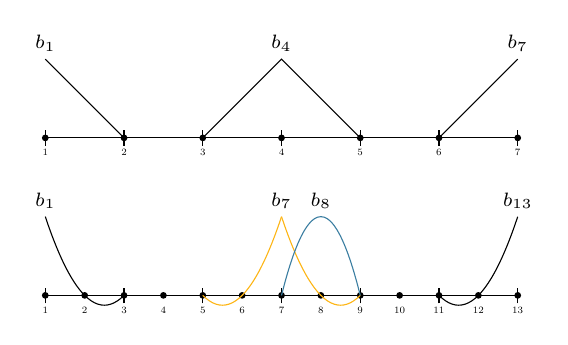
\begin{tikzpicture}
	\scriptsize
	\draw (0,-.1) grid (6,.1); 
	\foreach \i in {1,...,7}{
		\filldraw (\i-1,0) circle[radius=1pt] node[below=.1cm, scale=.5] {\i}; 
	}

	\draw (0,1) node[above] {$b_1$} -- (1,0); 
	\draw (5,0) -- (6,1) node[above] {$b_7$}; 
	\draw (2,0) -- (3,1) node[above] {$b_4$} -- (4,0); 

	% \begin{scope}[yshift=-2cm, xshift=-1cm]
	% 	\draw (0,-.075) grid (8,.075); 
	% 	\foreach \i in {1,...,8}{
	% 		\node[scale=.75] at (\i-.5,-.35) {$K_{\i}$}; 
	% 	}
	% 	\foreach[evaluate=\i as \x using (\i-1)*8/16] \i in {1,...,17}{
	% 		\filldraw (\x,0) circle[radius=1pt] node[below=.05cm, scale=.5] {\i}; 
	% 	}

	% 	% left boundary 
	% 	\draw[domain=0:1, smooth] plot(\x,{(\x-1)*(\x-.5)*2}); 
	% 	\node at (0,1.2) {$b_1$}; 
	% 	% right boundary 
	% 	\draw[domain=0:1, smooth, xshift=7cm] plot(\x,{\x*(\x-.5)*2}); 
	% 	\node at (8,1.2) {$b_{17}$}; 
	% 	% interior shape 
	% 	\draw[domain=0:1, smooth, xshift=2cm] plot(\x,{\x*(\x-.5)*2}); 		
	% 	\draw[domain=0:1, smooth, xshift=3cm] plot(\x,{(\x-1)*(\x-.5)*2}); 
	% 	\node at (3,1.2) {$b_{7}$}; 
	% 	% interior bubble 
	% 	\draw[domain=0:1, smooth, xshift=5cm] plot(\x,{\x*(1-\x)*4}); 
	% 	\node at (5.5,1.2) {$b_{12}$}; 
	% \end{scope}

	\begin{scope}[yshift=-2cm]
		\draw (0,-.1) grid (6,.1); 
		\foreach[evaluate=\i as \x using (\i-1)*6/12] \i in {1,...,13}{
			\filldraw (\x,0) circle[radius=1pt] node[below=.1cm, scale=.5] {\i}; 
		}
		% left boundary 
		\draw[domain=0:1, smooth] plot(\x,{(\x-1)*(\x-.5)*2}); 
		\node at (0,1.2) {$b_1$}; 

		% right boundary 
		\draw[domain=0:1, smooth, xshift=5cm] plot(\x,{\x*(\x-.5)*2}); 
		\node at (6,1.2) {$b_{13}$}; 

		% interior shape 
		\draw[domain=0:1, smooth, xshift=2cm, secondary] plot(\x,{\x*(\x-.5)*2}); 		
		\draw[domain=0:1, smooth, xshift=3cm, secondary] plot(\x,{(\x-1)*(\x-.5)*2}); 
		\node at (3,1.2) {$b_{7}$}; 

		% interior bubble 
		\draw[domain=0:1, smooth, xshift=3cm, founder] plot(\x,{\x*(1-\x)*4}); 
		\node at (3.5,1.2) {$b_{8}$}; 
	\end{scope}
\end{tikzpicture}
\end{document}